\documentclass[UTF8,openany,zihao=-4,oneside]{ctexbook}

% Page and typography
\usepackage[a4paper,top=23mm,bottom=24mm,left=24mm,right=24mm,headheight=15pt,headsep=8mm,footskip=12mm]{geometry}
\linespread{1.08}
\raggedbottom
\sloppy
\emergencystretch=3em

% Core packages
\usepackage{amsmath,amssymb,mathtools}
\usepackage{graphicx}
\graphicspath{{figures/}}
\usepackage{booktabs,longtable,array,tabularx,multirow,makecell}
\usepackage{enumitem}
\usepackage[table]{xcolor}
\usepackage{tikz}
\usetikzlibrary{positioning,arrows.meta,calc,fit,shapes.geometric}
\usepackage{caption}
\usepackage{float}
\usepackage{fancyhdr}
\usepackage{titlesec}
\usepackage{titletoc}
\usepackage{tocloft}
\usepackage[most]{tcolorbox}
\usepackage{listings}
\usepackage{etoolbox}
\usepackage{hyperref}
\usepackage{bookmark}

% Brand colors
\definecolor{FGBlue}{HTML}{1F4E79}
\definecolor{FGDeep}{HTML}{102A43}
\definecolor{FGCyan}{HTML}{2E8BC0}
\definecolor{FGOrange}{HTML}{D98A15}
\definecolor{FGGray}{HTML}{F3F6F9}
\definecolor{FGLine}{HTML}{D7E2EA}
\definecolor{FGText}{HTML}{243B53}

\hypersetup{
  colorlinks=true,
  linkcolor=FGBlue,
  urlcolor=FGCyan,
  citecolor=FGOrange,
  pdfauthor={FlameGuard},
  pdftitle={稳燃宝垃圾脱水实验设计手册},
  pdfsubject={垃圾干燥脱水实验、数据采集、干燥特性建模与控制参数标定},
  pdfkeywords={FlameGuard, 稳燃宝, 垃圾脱水, 干燥实验, 含水率, 预热控制}
}

% Paragraph and list tuning
\setlength{\parindent}{2em}
\setlength{\parskip}{0.18em}
\setlist{itemsep=0.15em,topsep=0.35em,leftmargin=2.2em}
\renewcommand{\arraystretch}{1.22}
\setlength{\tabcolsep}{5pt}
\setlength{\LTleft}{0pt}
\setlength{\LTright}{0pt}
\AtBeginEnvironment{longtable}{\small\renewcommand{\arraystretch}{1.2}}

% Pandoc compatibility and manual utilities
\providecommand{\tightlist}{\setlength{\itemsep}{0pt}\setlength{\parskip}{0pt}}
\providecommand{\passthrough}[1]{#1}
\newcommand{\manualdivider}{\par\vspace{0.6em}\noindent\textcolor{FGLine}{\rule{\linewidth}{0.7pt}}\vspace{0.6em}\par}
\newcommand{\pathcode}[1]{\texttt{\detokenize{#1}}}
\newcommand{\notebox}[2]{\begin{tcolorbox}[enhanced,colback=FGBlue!4,colframe=FGBlue!45,boxrule=0.5pt,arc=1.5mm,left=4mm,right=4mm,top=3mm,bottom=3mm]\sffamily\textbf{\color{FGDeep}#1}\par\vspace{0.25em}\color{FGText}#2\end{tcolorbox}}
\newcommand{\warnbox}[2]{\begin{tcolorbox}[enhanced,colback=FGOrange!6,colframe=FGOrange!55,boxrule=0.5pt,arc=1.5mm,left=4mm,right=4mm,top=3mm,bottom=3mm]\sffamily\textbf{\color{FGDeep}#1}\par\vspace{0.25em}\color{FGText}#2\end{tcolorbox}}

% Captions
\captionsetup{font=small,labelfont={bf,color=FGBlue},labelsep=quad}

% Chapter / section styles
\titleformat{\chapter}[display]
  {\Huge\bfseries\sffamily\color{FGDeep}}
  {\begin{tikzpicture}[baseline=(n.base)]\node[fill=FGBlue,text=white,rounded corners=1.5mm,inner xsep=8pt,inner ysep=5pt,font=\Large\bfseries\sffamily] (n) {第\thechapter 章};\end{tikzpicture}}
  {0.85em}
  {\Huge}
  [\vspace{0.35em}{\color{FGOrange}\titlerule[1.2pt]}]
\titlespacing*{\chapter}{0pt}{-4mm}{11mm}

\titleformat{\section}
  {\Large\bfseries\sffamily\color{FGBlue}}
  {\thesection}{0.75em}{}
  [\vspace{0.15em}{\color{FGLine}\titlerule[0.6pt]}]
\titlespacing*{\section}{0pt}{2.1ex plus .4ex}{1.1ex}

\titleformat{\subsection}
  {\large\bfseries\sffamily\color{FGDeep}}
  {\thesubsection}{0.75em}{}
\titlespacing*{\subsection}{0pt}{1.8ex plus .3ex}{0.8ex}

\titleformat{\subsubsection}
  {\normalsize\bfseries\sffamily\color{FGDeep}}
  {\thesubsubsection}{0.65em}{}
\titlespacing*{\subsubsection}{0pt}{1.3ex plus .2ex}{0.55ex}

% TOC styling
\renewcommand{\cftchapfont}{\sffamily\bfseries\color{FGDeep}}
\renewcommand{\cftsecfont}{\sffamily\color{FGText}}
\renewcommand{\cftchappagefont}{\sffamily\bfseries\color{FGBlue}}
\renewcommand{\cftsecpagefont}{\sffamily\color{FGText}}
\setlength{\cftbeforechapskip}{0.45em}

% Header / footer
\pagestyle{fancy}
\fancyhf{}
\fancyhead[L]{\sffamily\small\color{FGDeep}“稳燃宝”垃圾脱水实验设计手册}
\fancyhead[R]{\sffamily\small\color{FGBlue}\leftmark}
\fancyfoot[L]{\sffamily\scriptsize\color{FGText}实验系统 · 数据采集 · 干燥模型 · 控制接口}
\fancyfoot[R]{\sffamily\small\bfseries\color{FGBlue}\thepage}
\renewcommand{\headrulewidth}{0.5pt}
\renewcommand{\footrulewidth}{0pt}
\renewcommand{\headrule}{\hbox to\headwidth{\color{FGLine}\leaders\hrule height \headrulewidth\hfill}}
\fancypagestyle{plain}{%
  \fancyhf{}%
  \fancyfoot[R]{\sffamily\small\bfseries\color{FGBlue}\thepage}%
  \renewcommand{\headrulewidth}{0pt}%
}

% Code listings
\lstdefinestyle{fgcode}{
  basicstyle=\ttfamily\small,
  backgroundcolor=\color{FGGray},
  frame=single,
  rulecolor=\color{FGLine},
  framerule=0.5pt,
  breaklines=true,
  columns=fullflexible,
  keepspaces=true,
  showstringspaces=false,
  tabsize=2,
  xleftmargin=1em,
  xrightmargin=1em,
  framexleftmargin=0.6em,
  framexrightmargin=0.6em,
  aboveskip=0.8em,
  belowskip=0.8em
}
\lstset{style=fgcode}

% Inline badges, aligned with the other manuals
\newcommand{\fgbadge}[1]{\tcbox[colback=FGBlue!6,colframe=FGBlue!35,boxrule=0.4pt,arc=1mm,left=2pt,right=2pt,top=1pt,bottom=1pt,on line]{\sffamily\footnotesize #1}}

\begin{document}

\begin{titlepage}
\begin{tikzpicture}[remember picture,overlay]
  \fill[FGDeep] (current page.north west) rectangle ([yshift=-88mm]current page.north east);
  \fill[FGBlue] ([yshift=-88mm]current page.north west) rectangle ([yshift=-92mm]current page.north east);
  \fill[FGOrange] ([yshift=-92mm]current page.north west) rectangle ([yshift=-94mm]current page.north east);
  \fill[FGGray] ([yshift=-94mm]current page.north west) rectangle (current page.south east);
  \draw[FGBlue!20,line width=1.2pt] ([xshift=18mm,yshift=-122mm]current page.north west) -- ([xshift=-18mm,yshift=-122mm]current page.north east);
\end{tikzpicture}
\vspace*{13mm}
{\sffamily\bfseries\color{white}\fontsize{18}{22}\selectfont FlameGuard / 稳燃宝}\par
\vspace{9mm}
{\sffamily\bfseries\color{white}\fontsize{33}{40}\selectfont 垃圾脱水实验设计手册}\par
\vspace{4mm}
{\sffamily\color{white}\fontsize{15}{20}\selectfont 样品制备 · 称重采集 · 干燥曲线 · 控制参数标定}\par
\vspace{36mm}
\begin{tcolorbox}[enhanced,width=\textwidth,colback=white,colframe=FGLine,boxrule=0.7pt,arc=2mm,drop shadow={black!12!white},left=8mm,right=8mm,top=6mm,bottom=6mm]
{\sffamily\bfseries\Large\color{FGDeep}v0.2.0 Beta}\par\vspace{0.6em}
本手册由项目设计说明书中的“垃圾干燥特性实验设计”内容拆分、整理并扩展形成，采用与现有 FlameGuard 技术手册一致的版式、封面、页眉页脚和章节样式。
\end{tcolorbox}
\vfill
{\sffamily\small\color{FGText}炉火纯青队 · 大学生节能减排社会实践与科技竞赛 · 2025}\par
\end{titlepage}

\frontmatter
\pagestyle{plain}
\tableofcontents
\cleardoublepage
\pagestyle{fancy}
\mainmatter

\chapter{概述}

\section{实验手册定位}

本手册用于说明“稳燃宝”（FlameGuard）系统中垃圾脱水实验的设计目的、实验装置、样品体系、变量设置、数据采集、数据处理方法和控制模型接口。该实验是整个自适应控温预热系统的数据基础：通过可控温度下的连续称重实验，获得典型乡村生活垃圾组分的含水率衰减曲线，并进一步形成“垃圾组分占比--预热条件--脱水效果”的参数库。

\notebox{实验目标}{通过多组分、不同温度条件下的脱水实验，定量回答三个问题：第一，不同垃圾组分的初始湿基含水率有多大差异；第二，不同温度下达到目标含水率需要多长时间；第三，组分占比变化如何影响预热炉控制器对烟气温度和烟气流速的设定。}

从系统角度看，本实验位于“来料识别--预热控制--稳燃验证”的前端。实验输出不直接控制焚烧炉，而是为预热炉模型、内层优化器和控制器提供干燥动力学参数。图 \ref{fig:experiment-to-control} 给出了实验数据进入稳燃宝控制系统的关系。

\begin{figure}[htbp]
\centering
\begin{tikzpicture}[
  node distance=8mm and 8mm,
  box/.style={draw=FGBlue,fill=FGBlue!6,very thick,rounded corners=2mm,minimum height=11mm,text width=30mm,align=center,font=\sffamily\small},
  orangebox/.style={draw=FGOrange,fill=FGOrange!8,very thick,rounded corners=2mm,minimum height=11mm,text width=32mm,align=center,font=\sffamily\small},
  arrow/.style={-{Latex[length=2.8mm,width=2mm]},very thick,FGBlue!80},
  feedback/.style={-{Latex[length=2.8mm,width=2mm]},very thick,FGOrange!85,dashed}
]
\node[box] (sample) {典型垃圾样品\\组分与配比};
\node[box, right=of sample] (test) {烘箱脱水实验\\连续称重};
\node[box, right=of test] (curve) {干燥曲线\\$\omega(t,T)$};
\node[orangebox, below=15mm of curve] (param) {干燥参数库\\$\omega_0,t_{ref},s$};
\node[box, left=of param] (model) {预热炉模型\\停留时间/热量需求};
\node[box, left=of model] (ctrl) {控制器/优化器\\$T_g,v_g$ 决策};
\draw[arrow] (sample) -- (test);
\draw[arrow] (test) -- (curve);
\draw[arrow] (curve) -- (param);
\draw[arrow] (param) -- (model);
\draw[arrow] (model) -- (ctrl);
\draw[feedback] (ctrl.north) |- node[pos=0.24, left, font=\scriptsize\sffamily] {预热目标} (test.south);
\end{tikzpicture}
\caption{垃圾脱水实验数据与预热控制系统的接口关系}
\label{fig:experiment-to-control}
\end{figure}

\section{核心实验结论}

根据已完成实验，典型生活垃圾组分在初始湿基含水率、脱水速率和温度敏感性上存在明显差异。菜叶和西瓜皮的初始湿基含水率接近或超过 94\%，米饭约 61\%，肉类样品最低；在 175\,\textdegree C 附近，肉类样品达到 80\% 去除率所需时间较短，西瓜皮较长；升温能够缩短脱水时间，其中西瓜皮对温度变化更敏感。

\warnbox{设计含义}{预热控制不宜采用单一“平均垃圾”假设。控制器需要根据组分占比预测等效含水率和等效干燥时间；对于高西瓜皮、高菜叶等高湿工况，应提前提高预热强度或延长等效停留时间；对于肉类占比较高或初始含水率较低的工况，应防止过度预热导致碳化、阴燃或能耗浪费。}

\manualdivider

\chapter{实验对象与样品体系}

\section{样品选择原则}

实验对象以乡村生活垃圾中占比高、对焚烧稳定性影响大的高湿厨余垃圾为核心。说明书中选取的代表性组分包括菜叶、西瓜皮、橘子皮、米饭和熟肉，并设置混合样验证单组分模型向实际混合垃圾的外推能力。

样品选择遵循以下原则：

\begin{enumerate}
\item \textbf{高湿代表性}：优先选择含水率高、干燥过程对预热负荷影响显著的厨余组分。
\item \textbf{热工差异性}：同时覆盖纤维类、淀粉类、果皮类和蛋白/脂肪类组分，以观察不同传热传质响应。
\item \textbf{工程可测性}：样品质量、尺寸和形态应适合烘箱内托盘称重，保证称重信号连续稳定。
\item \textbf{控制可转译性}：最终实验指标应能转化为控制器可用的参数，如初始含水率、目标含水率所需时间和温度敏感性系数。
\end{enumerate}

\section{混合样配比}

为模拟乡村厨余垃圾的典型入炉状态，混合样按表 \ref{tab:mix-ratio} 的质量占比配置。该配比用于验证单组分干燥规律的线性叠加是否能够近似描述混合垃圾脱水过程。

\begin{table}[htbp]
\centering
\begin{tabularx}{0.86\textwidth}{p{30mm}p{28mm}X}
\toprule
组分 & 质量占比 & 设计作用 \\
\midrule
菜叶 & 30\% & 高湿叶菜类组分，代表厨余中含水量高且薄层传热较快的部分。\\
西瓜皮 & 20\% & 高湿果皮类组分，代表厚壁组织和较慢扩散过程。\\
橘子皮 & 10\% & 果皮类组分，兼具纤维结构和表皮阻水特征。\\
米饭 & 25\% & 淀粉类熟食组分，代表剩饭剩菜中较常见的热质传递特征。\\
肉类 & 15\% & 蛋白/脂肪类组分，初始含水率相对较低，用于检验过热风险。\\
\bottomrule
\end{tabularx}
\caption{典型乡村厨余垃圾混合样配比}
\label{tab:mix-ratio}
\end{table}

\manualdivider

\chapter{实验系统与仪器配置}

\section{实验系统组成}

实验系统由台式烘箱、实时在线电子天平、挂钩/托盘连接结构、数据采集电脑和串口采集软件组成。台式烘箱提供恒温环境，电子天平在不打断加热过程的条件下连续记录样品质量，数据采集电脑保存质量--时间序列。

\begin{figure}[htbp]
\centering
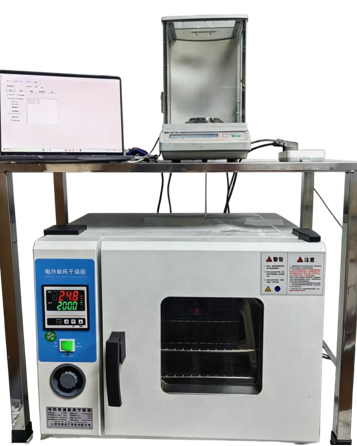
\includegraphics[width=0.78\textwidth]{fig_experiment_setup.png}
\caption{实验装置现场图：烘箱、电子天平、挂钩托盘和电脑采集系统}
\label{fig:experiment-setup}
\end{figure}

图 \ref{fig:experiment-setup} 中，挂钩用于连接电子天平与烘箱内托盘；烘箱用于控制恒温环境并烘干样品水分；电脑通过数据线连接电子天平，实时采集、传输和记录称重数据；电子天平精度为 0.001\,g，用于记录样品质量随时间的变化。

\section{关键仪器参数}

\begin{table}[htbp]
\centering
\begin{tabularx}{\textwidth}{p{28mm}p{36mm}X}
\toprule
模块 & 关键参数 & 功能说明 \\
\midrule
台式烘箱 & 控温精度约 0.1\,\textdegree C & 提供 125--215\,\textdegree C 范围内的恒温干燥环境，模拟预热烟气可用温区。\\
在线电子天平 & 分辨率 0.001\,g & 通过挂钩与托盘连接，实现加热过程中不取样连续称重。\\
数据采集软件 & 采样间隔约 1000\,ms & 将天平串口数据实时记录为质量--时间序列，用于绘制干燥曲线。\\
挂钩/托盘系统 & 金属挂钩、轻质托盘 & 保持样品悬挂稳定，降低烘箱振动和空气扰动对称重信号的影响。\\
\bottomrule
\end{tabularx}
\caption{垃圾脱水实验系统关键仪器配置}
\label{tab:equipment}
\end{table}

\begin{figure}[htbp]
\centering
\begin{minipage}{0.47\textwidth}
\centering
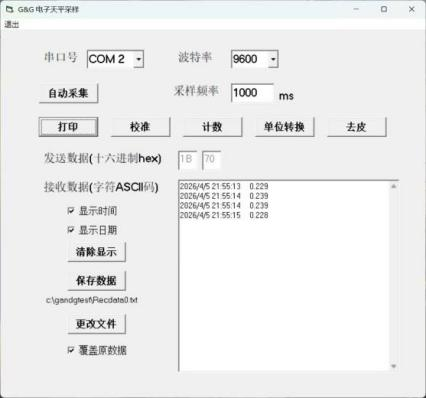
\includegraphics[width=\textwidth]{fig_balance_ui.jpeg}
\end{minipage}\hfill
\begin{minipage}{0.47\textwidth}
\centering
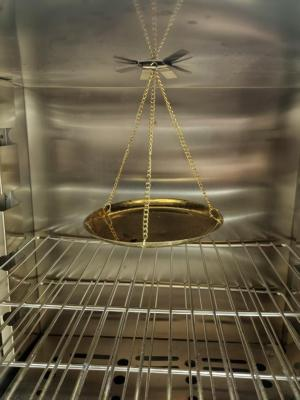
\includegraphics[width=\textwidth]{fig_oven_inside.jpeg}
\end{minipage}
\caption{电子天平数据采集界面（左）与烘箱内部挂钩/托盘安装图（右）}
\label{fig:balance-and-oven}
\end{figure}

\section{实验装置检查清单}

每组实验开始前，应完成以下检查：

\begin{enumerate}
\item 烘箱预热至目标温度并稳定至少 5\,min，记录温度设定值和实际显示值。
\item 电子天平调零，确认挂钩和托盘在烘箱关门后不接触内壁或搁架。
\item 数据采集软件串口、波特率和采样间隔设置正确，并保存到独立数据文件。
\item 样品装盘后确认质量读数无明显漂移，关闭烘箱门后再开始正式记录。
\item 实验过程中不打开炉门、不移动线缆、不触碰桌面，减少称重信号突变。
\end{enumerate}

\manualdivider

\chapter{变量设计与实验工况}

\section{控制变量法设计}

本实验采用控制变量法，以加热温度和加热时间为核心控制变量。单组分样品先进行完整干燥曲线测试，混合样再用于交叉验证。说明书原始设计中设置 125\,\textdegree C、150\,\textdegree C、175\,\textdegree C 三组温度梯度；后续数据表中进一步包含 200\,\textdegree C 和米饭 215\,\textdegree C 的高温补充工况，用于评估温度敏感性和高温加速脱水趋势。

\begin{table}[htbp]
\centering
\begin{tabularx}{\textwidth}{p{32mm}p{42mm}X}
\toprule
变量类别 & 设置范围 & 说明 \\
\midrule
垃圾组分 & 菜叶、西瓜皮、橘子皮、米饭、肉类、混合样 & 覆盖乡村厨余垃圾中高湿植物类、果皮类、淀粉类和蛋白类组分。\\
加热温度 & 125、150、175、200、215\,\textdegree C & 125--175\,\textdegree C 为基础梯度；200--215\,\textdegree C 为温度响应补充工况。\\
加热时间 & 至样品质量趋于稳定或达到目标含水率 & 用连续称重曲线自动识别关键时间点。\\
重复次数 & 每组实验重复 3 次后取平均值 & 用于削弱样品差异、称重扰动和偶然误差。\\
输出指标 & 初始湿基含水率、到 0\% 含水率时间、到 52.35\% 含水率时间 & 用于构建控制器和预热炉模型可调用的数据表。\\
\bottomrule
\end{tabularx}
\caption{脱水实验变量与工况设计}
\label{tab:variables}
\end{table}

\section{现场样品记录}

图 \ref{fig:field-samples} 为部分现场实验样品结果。从左到右、从上到下依次包括米饭 200\,\textdegree C、米饭 225\,\textdegree C、西瓜皮 175\,\textdegree C、西瓜皮 200\,\textdegree C、混合样 150\,\textdegree C、肉类 125\,\textdegree C、肉类 150\,\textdegree C、橘皮 150\,\textdegree C、橘皮 175\,\textdegree C 等样品状态。

\begin{figure}[htbp]
\centering
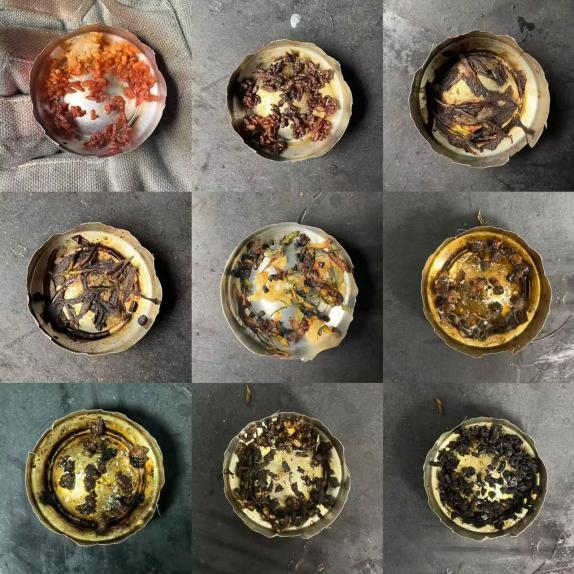
\includegraphics[width=0.76\textwidth]{fig_field_samples.jpeg}
\caption{现场实验样品结果记录}
\label{fig:field-samples}
\end{figure}

\manualdivider

\chapter{实验流程与操作规范}

\section{标准实验流程}

每一个“组分--温度”组合均按照同一流程执行，以保证数据可比性。

\begin{enumerate}
\item \textbf{样品准备}：将待测垃圾组分切分为大小接近的小块，去除不可代表的极端杂质，称量初始净重 $m_0$。
\item \textbf{设备预热}：将烘箱调至目标温度，待温度稳定后安装托盘与挂钩，并确认空载质量读数稳定。
\item \textbf{开始记录}：将样品放入托盘，关闭烘箱门，启动串口采集程序，记录时间 $t$ 和质量 $m(t)$。
\item \textbf{连续干燥}：实验过程中保持烘箱封闭，直到样品质量变化趋于平缓或达到预设终止条件。
\item \textbf{结束称量}：记录结束净重 $m_d$，作为干基质量的实验近似值。
\item \textbf{数据保存}：按“组分--温度--重复编号”的命名规则保存原始数据和处理数据。
\item \textbf{重复实验}：同一工况至少重复 3 次，取均值并记录标准差或最大偏差。
\end{enumerate}

\section{质量控制}

\warnbox{称重数据异常处理}{若曲线中出现由于开门、碰线、托盘摆动导致的瞬时跳点，应在原始数据中标注，并在处理数据中采用局部剔除或中值滤波。不得直接修改原始采集文件。}

质量控制重点包括：样品切分尺寸尽量一致；同一组分实验尽量使用同批次样品；烘箱温度达到设定值后再开始正式计时；样品盘和挂钩不应触碰烘箱内壁；所有实验数据应保留原始文件、处理脚本和图像结果，便于复核。

\manualdivider

\chapter{数据处理与指标定义}

\section{湿基含水率计算}

以连续称重得到的样品质量 $m(t)$ 和结束净重 $m_d$ 为基础，湿基含水率定义为

\begin{equation}
\omega(t)=\frac{m(t)-m_d}{m(t)}\times 100\% .
\label{eq:wet-basis-moisture}
\end{equation}

其中，$m_d$ 为实验结束时的近似干基质量。初始湿基含水率为

\begin{equation}
\omega_0=\frac{m_0-m_d}{m_0}\times 100\% .
\label{eq:initial-moisture}
\end{equation}

若需要计算水分去除率，可采用

\begin{equation}
\eta(t)=\frac{m_0-m(t)}{m_0-m_d}\times 100\% .
\label{eq:removal-ratio}
\end{equation}

当 $\eta(t)=80\%$ 时对应的时间记为 $t_{80}$。该指标可用于比较不同组分在相同温度下的脱水速度。

\section{目标含水率时间}

实验数据表中记录了两个关键时间：到 0\% 含水率时间和到 52.35\% 含水率时间。前者代表样品质量趋近干基状态所需的时间，可作为最大干燥难度指标；后者用于描述从高湿状态下降到工程目标附近时的脱水速度。

在控制系统中，目标含水率不一定固定为 52.35\%。实际目标由治理器根据炉膛温度、安全边界和稳燃区间动态生成。实验数据的作用是为任意目标含水率插值或拟合提供基础曲线。

\section{干燥曲线拟合}

对每条实验曲线，建议至少保存以下三类结果：

\begin{enumerate}
\item 原始质量曲线 $m(t)$；
\item 湿基含水率曲线 $\omega(t)$；
\item 关键时间点，如 $t_{80}$、$t_{52.35}$、$t_{0}$ 或达到控制目标含水率所需时间。
\end{enumerate}

对于控制器使用的低阶参数库，可以用线性或分段线性方式近似描述温度对干燥时间的影响：

\begin{equation}
 t_i(T)=t_{ref,i}+s_i\left(T-T_{ref}\right),
\label{eq:temperature-sensitivity}
\end{equation}

其中，$i$ 表示垃圾组分，$T_{ref}$ 可取 175\,\textdegree C，$t_{ref,i}$ 为参考温度下达到目标脱水程度所需时间，$s_i$ 为温度敏感性系数。

\manualdivider

\chapter{实验结果与干燥特性数据库}

\section{原始实验数据表}

表 \ref{tab:raw-results} 整理了设计说明书附件中的不同组分生活垃圾干燥特性实验结果。该表是后续曲线绘制、参数拟合和控制器数据库构建的基础。

{\scriptsize
\setlength{\tabcolsep}{2pt}
\begin{longtable}{@{}p{15mm}p{14mm}p{18mm}p{18mm}p{20mm}p{24mm}p{27mm}@{}}
\caption{不同组分生活垃圾干燥特性实验结果}\label{tab:raw-results}\\
\toprule
\makecell{垃圾\\组分} & \makecell{实验\\温度/\textdegree C} & \makecell{初始\\净重/g} & \makecell{结束\\净重/g} & \makecell{湿基\\含水率/\%} & \makecell{到 0\% 含水率\\时间/min} & \makecell{到 52.35\% 含水率\\时间/min} \\
\midrule
\endfirsthead
\toprule
\makecell{垃圾\\组分} & \makecell{实验\\温度/\textdegree C} & \makecell{初始\\净重/g} & \makecell{结束\\净重/g} & \makecell{湿基\\含水率/\%} & \makecell{到 0\% 含水率\\时间/min} & \makecell{到 52.35\% 含水率\\时间/min} \\
\midrule
\endhead
橘子皮 & 150 & 7.867 & 1.492 & 81.03 & 32.88 & 18.88 \\
橘子皮 & 175 & 8.070 & 1.464 & 81.86 & 26.90 & 14.26 \\
橘子皮 & 200 & 7.703 & 1.369 & 82.23 & 17.08 & 10.54 \\
米饭 & 150 & 11.562 & 4.698 & 59.37 & 45.90 & 8.59 \\
米饭 & 175 & 9.569 & 3.601 & 62.37 & 28.40 & 7.29 \\
米饭 & 200 & 10.153 & 3.893 & 61.66 & 24.67 & 5.60 \\
米饭 & 215 & 8.656 & 3.375 & 61.01 & 16.83 & 3.60 \\
肉类 & 125 & 7.022 & 4.568 & 34.95 & 46.13 & 0.00 \\
肉类 & 150 & 5.969 & 3.415 & 42.79 & 23.03 & 0.00 \\
肉类 & 175 & 6.098 & 3.180 & 47.85 & 17.95 & 0.00 \\
肉类 & 200 & 5.864 & 2.853 & 51.35 & 17.57 & 0.00 \\
菜叶 & 125 & 5.112 & 0.366 & 92.84 & 31.87 & 22.60 \\
菜叶 & 150 & 3.885 & 0.185 & 95.24 & 22.10 & 16.23 \\
菜叶 & 175 & 5.183 & 0.124 & 97.61 & 21.48 & 19.06 \\
菜叶 & 200 & 4.687 & 0.300 & 93.60 & 13.47 & 9.85 \\
西瓜皮 & 150 & 8.694 & 0.476 & 94.52 & 43.50 & 32.63 \\
西瓜皮 & 175 & 8.925 & 0.509 & 94.30 & 31.28 & 22.84 \\
西瓜皮 & 200 & 8.932 & 0.398 & 95.54 & 22.65 & 17.32 \\
混合样 & 150 & 10.137 & 2.232 & 77.98 & 40.82 & 19.14 \\
混合样 & 175 & 10.006 & 2.319 & 76.82 & 30.13 & 13.19 \\
混合样 & 200 & 9.976 & 2.290 & 77.04 & 24.10 & 10.29 \\
\bottomrule
\end{longtable}
}

\section{干燥曲线结果}

不同温度下的干燥曲线表明，垃圾含水率随加热时间延长呈现“先快速下降、后趋于平缓”的变化规律。加热温度越高，脱水速率越快，达到同一目标含水率所需时间越短。单组分和混合样的交叉验证进一步表明，不同组分对整体干燥速率的贡献不同，不能用单一常数描述全部垃圾工况。

\begin{figure}[htbp]
\centering
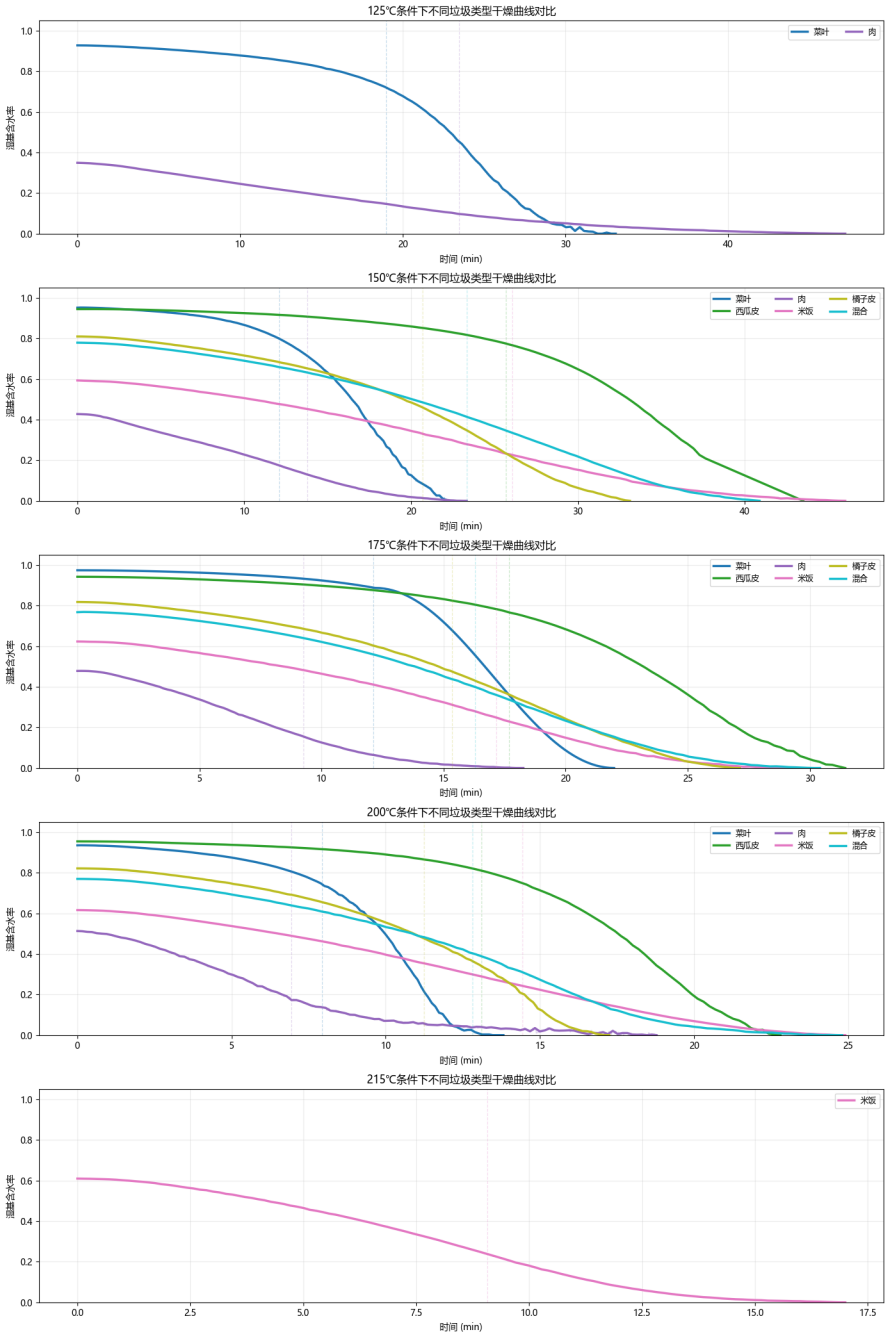
\includegraphics[width=0.76\textwidth]{fig_drying_curves_temperature.png}
\caption{各温度下不同种类垃圾干燥曲线对比}
\label{fig:drying-curves-temperature}
\end{figure}

\begin{figure}[htbp]
\centering
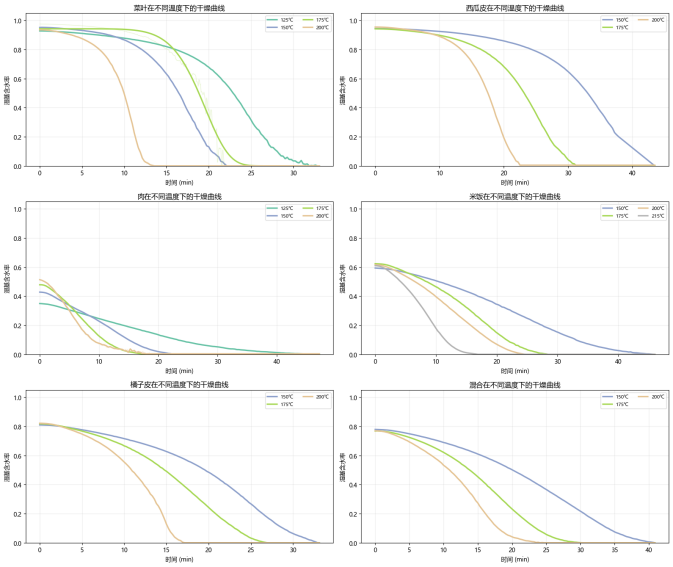
\includegraphics[width=0.86\textwidth]{fig_drying_curves_groups.png}
\caption{各实验组干燥特性曲线}
\label{fig:drying-curves-groups}
\end{figure}

\section{参数化结果}

从实验结果可提取控制器所需的三个核心参数：初始湿基含水率 $\omega_i$、参考干燥时间 $t_{ref,i}$ 和温度敏感性系数 $s_i$。表 \ref{tab:kinetic-param} 给出了说明书附件中已整理的典型参数。

\begin{table}[htbp]
\centering\footnotesize
\begin{tabularx}{\textwidth}{p{16mm}p{20mm}p{28mm}p{44mm}X}
\toprule
组分编号 & 组分名称 & 初始湿基含水率 $\omega_i$ & 175\,\textdegree C 下 20\% 含水率干燥时间 $t_{ref,i}$/min & 温度敏感性系数 $s_i$/(min/\textdegree C) \\
\midrule
$x_1$ & 菜叶 & 0.948 & 12.1 & -0.132 \\
$x_2$ & 西瓜皮 & 0.948 & 17.7 & -0.251 \\
$x_3$ & 橘子皮 & 0.817 & 15.3 & -0.189 \\
$x_4$ & 肉类 & 0.442 & 11.5 & -0.216 \\
$x_5$ & 混合样 & 0.773 & 16.3 & -0.210 \\
$x_6$ & 米饭 & 0.611 & 15.8 & -0.243 \\
\bottomrule
\end{tabularx}
\caption{典型厨余垃圾干燥特性参数}
\label{tab:kinetic-param}
\end{table}

\begin{figure}[htbp]
\centering
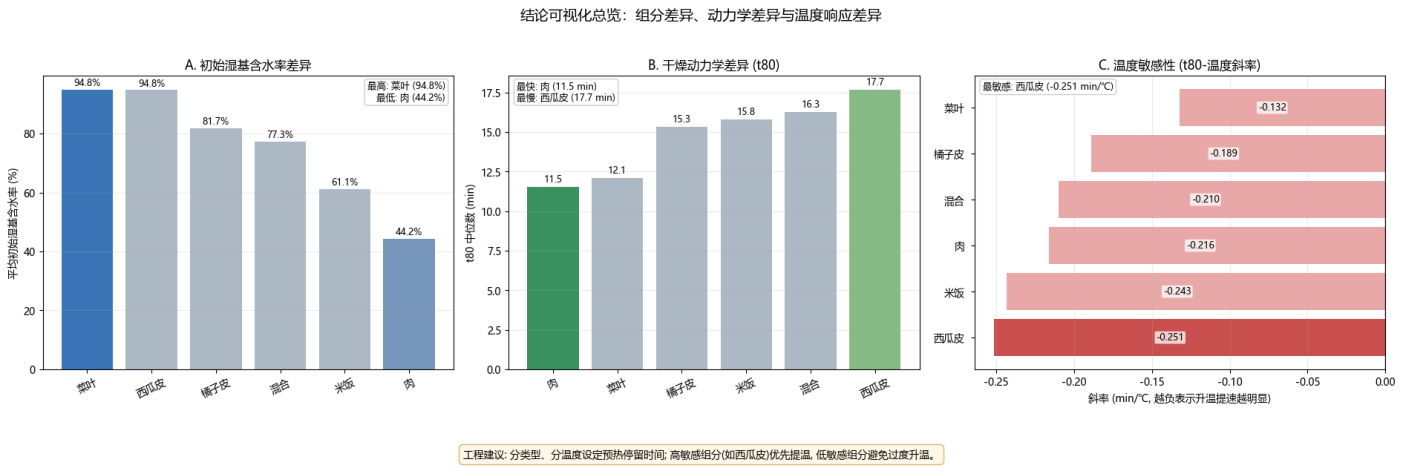
\includegraphics[width=0.92\textwidth]{fig_conclusion_analysis.png}
\caption{结论可视化分析：组分差异、动力学差异与温度响应差异}
\label{fig:conclusion-analysis}
\end{figure}

实验结论可以概括为：菜叶平均初始湿基含水率最高，约为 94.8\%；肉类样品相对较低，约为 44.2\%；按 $t_{80}$ 中位数统计，肉类样品干燥速度较快，西瓜皮样品较慢；温度敏感性分析显示，升温总体上能够加快干燥过程，但不同组分响应强度不同，西瓜皮对温度最敏感。

\manualdivider

\chapter{与控制系统的接口}

\section{输出给预热炉模型的参数}

垃圾脱水实验并不直接输出执行器命令，而是输出预热炉模型和控制器可调用的数据结构。推荐接口字段如表 \ref{tab:control-interface} 所示。

\begin{table}[htbp]
\centering
\begin{tabularx}{\textwidth}{p{32mm}p{36mm}X}
\toprule
字段 & 建议符号/单位 & 控制用途 \\
\midrule
组分质量占比 & $x_i$，无量纲 & 用于计算混合垃圾等效含水率、等效参考干燥时间和等效温度敏感性。\\
初始湿基含水率 & $\omega_i$，无量纲或 \% & 用于预测入口垃圾水分负荷和蒸发潜热需求。\\
参考干燥时间 & $t_{ref,i}$，min & 用于判断给定停留时间和温度下是否能达到目标含水率。\\
温度敏感性系数 & $s_i$，min/\textdegree C & 用于将实验温度梯度外推到预热烟气等效温度。\\
目标含水率时间 & $t_{target}$，min & 用于内层优化器约束预热炉停留时间和预热强度。\\
\bottomrule
\end{tabularx}
\caption{脱水实验结果到控制系统的推荐接口字段}
\label{tab:control-interface}
\end{table}

\section{混合垃圾等效性质}

若前端识别系统给出不同垃圾组分的质量占比 $x_i$，且满足

\begin{equation}
\sum_i x_i = 1, \quad x_i \ge 0,
\label{eq:ratio-sum}
\end{equation}

则混合垃圾等效初始含水率、等效参考干燥时间和等效温度敏感性可按质量加权计算：

\begin{align}
\omega_{mix} &= \sum_i x_i\omega_i, \\
t_{ref,mix} &= \sum_i x_i t_{ref,i}, \\
s_{mix} &= \sum_i x_i s_i.
\end{align}

在更精细的工程实现中，还应叠加样品粒径、堆积厚度、通风状态、预热炉停留时间和烟气侧换热系数等因素。若现场数据与实验室烘箱结果存在系统偏差，应通过运行数据重新标定 $t_{ref,i}$ 和 $s_i$。

\section{控制器使用方式}

控制器可按以下流程调用实验数据库：

\begin{enumerate}
\item 根据垃圾识别结果得到组分占比 $x_i$ 和入口垃圾估计含水率。
\item 计算混合等效参数 $\omega_{mix}$、$t_{ref,mix}$ 和 $s_{mix}$。
\item 由治理器给出目标出口含水率 $\omega^\star$。
\item 内层优化器在烟气温度、烟气流速、停留时间和资源约束下求解可行预热工况。
\item 若烟气余热不足，则计算辅助补热缺口；若预热温度或垃圾层温度触及安全边界，则降低预热强度或触发安全保护。
\end{enumerate}

\manualdivider

\chapter{安全边界与后续补充实验}

\section{安全边界}

垃圾脱水实验服务于工程预热控制，因此必须避免将实验结论误用到危险工况。建议保留以下安全边界：

\begin{enumerate}
\item 预热温度不应超过控制模型设定的环保与安全上限，防止二恶英前驱体生成和料斗阴燃风险。
\item 垃圾层等效温度应低于阴燃和碳化风险阈值，控制系统中可取 110\,\textdegree C 作为保护上限。
\item 实验室烘箱为静态小样本条件，工程预热炉存在堆积厚度、混合、通风和换热不均匀问题，直接外推时需要安全裕度。
\item 肉类等低初始含水率组分达到 52.35\% 目标含水率时间为 0，说明其初始含水率已低于该目标；工程控制中不应对这类组分进行额外强脱水。
\end{enumerate}

\section{建议补充实验}

为使实验数据库更适合工程落地，建议后续补充以下实验：

\begin{enumerate}
\item 增加相同温度下的重复样本数量，给出均值、标准差和置信区间。
\item 在 100--250\,\textdegree C 范围内补齐温度梯度，尤其是 125\,\textdegree C 以下的低温预热工况。
\item 增加不同颗粒尺寸、不同堆积厚度和不同通风速度下的干燥曲线。
\item 将烘箱实验结果与预热炉小试结果进行对比，建立实验室条件到工程预热炉条件的修正系数。
\item 增加目标含水率 30\%--35\% 区间的关键时间插值，以更直接服务于稳燃控制目标。
\end{enumerate}

\chapter{附录：文件与图像来源说明}

本手册中的图 \ref{fig:experiment-setup} 至图 \ref{fig:conclusion-analysis} 由设计说明书的 Word 文档中拆分提取，并按用途重命名后置于 \pathcode{figures/} 目录。表 \ref{tab:raw-results} 来自说明书附件“不同组分生活垃圾干燥特性实验结果数据表”。手册版式、封面风格、色彩、页眉页脚、目录与章节格式与 FlameGuard 现有技术手册保持一致。

\end{document}
